\documentclass[aspectratio=169]{beamer}
\usepackage{tikz}
\usepackage{xcolor}
\usepackage{amsmath}
\usepackage{amssymb}
\usepackage{listings}
\usetikzlibrary{shapes.geometric, arrows.meta, positioning, fit, backgrounds, shadows, decorations.pathreplacing, calc, matrix}

% Theme
\usetheme{Madrid}
\usecolortheme{beaver}

% Remove footer
\setbeamertemplate{footline}{}
\setbeamertemplate{navigation symbols}{}

% Custom colors
\definecolor{frontend}{RGB}{70, 130, 180}      % Steel blue
\definecolor{execution}{RGB}{60, 179, 113}     % Medium sea green
\definecolor{detection}{RGB}{220, 20, 60}      % Crimson
\definecolor{verification}{RGB}{148, 0, 211}   % Dark violet
\definecolor{oracle}{RGB}{255, 140, 0}         % Dark orange
\definecolor{lightgray}{RGB}{240, 240, 240}    % Light background

% Code listing style
\lstset{
    basicstyle=\ttfamily\tiny,
    keywordstyle=\color{blue},
    commentstyle=\color{gray},
    stringstyle=\color{red},
    showstringspaces=false,
    breaklines=true,
    frame=single,
    backgroundcolor=\color{lightgray}
}

\title{PythonFromScratch}
\subtitle{Scalable Static Analysis via Symbolic Execution \& Barrier Certificates}
\author{Technical Deep Dive}
\date{\today}

\begin{document}

% ============================================================================
% TITLE SLIDE
% ============================================================================
\begin{frame}[plain,noframenumbering]
\titlepage
\vspace{-0.5cm}
\begin{center}
\footnotesize
\textbf{Goal:} Sound bug detection for Python at scale\\
\textbf{Approach:} Z3-based symbolic execution + 5-layer barrier synthesis\\
\textbf{Result:} 67 bug types, 31 true positives in DeepSpeed (700 files)
\end{center}
\end{frame}

% ============================================================================
% SLIDE: Architecture Overview - Technical
% ============================================================================
\begin{frame}{System Architecture: 4-Stage Pipeline}
\vspace{-0.4cm}

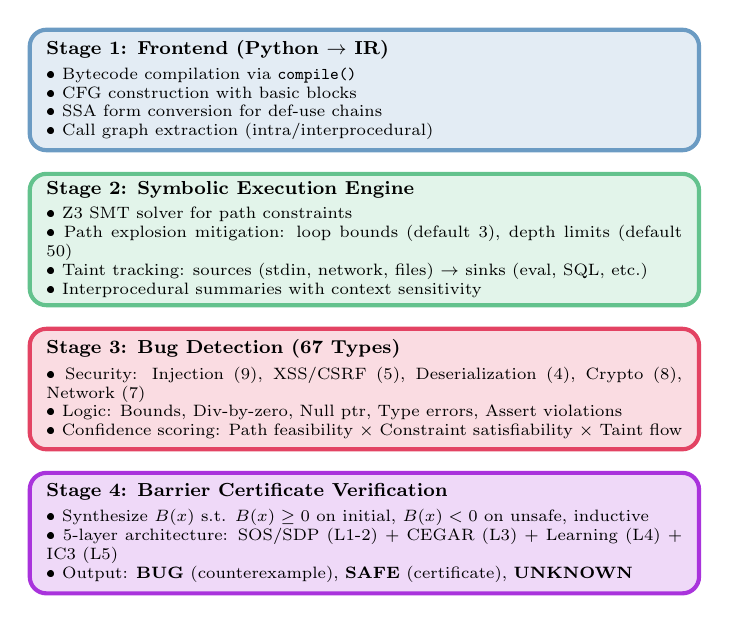
\begin{tikzpicture}[
    scale=0.85,
    transform shape,
    stage/.style={rectangle, rounded corners=6pt, draw, line width=1.5pt, 
                  minimum width=10cm, minimum height=1.8cm, align=left, font=\footnotesize},
    component/.style={rectangle, rounded corners=3pt, draw, line width=1pt,
                     minimum width=2.2cm, minimum height=0.6cm, align=center, font=\scriptsize}
]

% Stage 1: Frontend
\node[stage, fill=frontend!15, draw=frontend!80] (frontend) at (0, 3) {
    \textbf{Stage 1: Frontend (Python $\rightarrow$ IR)}\\[0.1cm]
    \begin{minipage}{9.5cm}
    \scriptsize
    • Bytecode compilation via \texttt{compile()}\\
    • CFG construction with basic blocks\\
    • SSA form conversion for def-use chains\\
    • Call graph extraction (intra/interprocedural)
    \end{minipage}
};

% Stage 2: Symbolic Execution
\node[stage, fill=execution!15, draw=execution!80, below=0.3cm of frontend] (symbolic) {
    \textbf{Stage 2: Symbolic Execution Engine}\\[0.1cm]
    \begin{minipage}{9.5cm}
    \scriptsize
    • Z3 SMT solver for path constraints\\
    • Path explosion mitigation: loop bounds (default 3), depth limits (default 50)\\
    • Taint tracking: sources (stdin, network, files) $\rightarrow$ sinks (eval, SQL, etc.)\\
    • Interprocedural summaries with context sensitivity
    \end{minipage}
};

% Stage 3: Bug Detection
\node[stage, fill=detection!15, draw=detection!80, below=0.3cm of symbolic] (detection) {
    \textbf{Stage 3: Bug Detection (67 Types)}\\[0.1cm]
    \begin{minipage}{9.5cm}
    \scriptsize
    • Security: Injection (9), XSS/CSRF (5), Deserialization (4), Crypto (8), Network (7)\\
    • Logic: Bounds, Div-by-zero, Null ptr, Type errors, Assert violations\\
    • Confidence scoring: Path feasibility $\times$ Constraint satisfiability $\times$ Taint flow
    \end{minipage}
};

% Stage 4: Verification
\node[stage, fill=verification!15, draw=verification!80, below=0.3cm of detection] (verification) {
    \textbf{Stage 4: Barrier Certificate Verification}\\[0.1cm]
    \begin{minipage}{9.5cm}
    \scriptsize
    • Synthesize $B(x)$ s.t. $B(x) \geq 0$ on initial, $B(x) < 0$ on unsafe, inductive\\
    • 5-layer architecture: SOS/SDP (L1-2) + CEGAR (L3) + Learning (L4) + IC3 (L5)\\
    • Output: \textbf{BUG} (counterexample), \textbf{SAFE} (certificate), \textbf{UNKNOWN}
    \end{minipage}
};

\end{tikzpicture}

\end{frame}

% ============================================================================
% SLIDE: Z3 Integration - Part 1
% ============================================================================
\begin{frame}{Z3 SMT Solver: Symbolic State}
\vspace{-0.2cm}

\begin{block}{Symbolic State}
\Large
\[
\Sigma = \langle \text{pc}, \sigma, \pi, \tau \rangle
\]
\end{block}

\vspace{0.5cm}

\begin{block}{Components}
\large
• $\text{pc}$: path condition (Z3 formula)

\vspace{0.3cm}
• $\sigma$: symbolic store (variables)

\vspace{0.3cm}
• $\pi$: heap model (objects)

\vspace{0.3cm}
• $\tau$: taint tracking map
\end{block}

\end{frame}

% ============================================================================
% SLIDE: Z3 Example
% ============================================================================
\begin{frame}{Z3 SMT Solver: Example}
\vspace{-0.2cm}

\begin{block}{Code}
\Large
\texttt{if x > 0: y = 1 / x}
\end{block}

\vspace{0.5cm}

\begin{block}{Analysis}
\large
Path condition: $\text{pc} = (x > 0)$

\vspace{0.4cm}
Bug condition: $(x = 0)$

\vspace{0.4cm}
Z3 query: Is $(x > 0) \land (x = 0)$ satisfiable?

\vspace{0.4cm}
\textbf{Result:} UNSAT $\Rightarrow$ Safe!
\end{block}

\end{frame}

% ============================================================================
% SLIDE: Z3 Solver Strategies
% ============================================================================
\begin{frame}{Z3: Solver Strategies}
\vspace{-0.2cm}

\begin{block}{Incremental Solving}
\Large
• Use \texttt{push()}/\texttt{pop()} for branches

\vspace{0.3cm}
• Reuse constraint context

\vspace{0.3cm}
• Avoid redundant work
\end{block}

\vspace{0.5cm}

\begin{block}{Theory Selection}
\Large
• Bit-vectors for integers

\vspace{0.3cm}
• Array theory for collections

\vspace{0.3cm}
• Quantifiers for loops
\end{block}

\end{frame}

% ============================================================================
% SLIDE: Z3 Performance
% ============================================================================
\begin{frame}{Z3: Performance Management}
\vspace{-0.2cm}

\begin{block}{Timeout Strategy}
\Large
• Per-query timeout: 5 seconds

\vspace{0.3cm}
• Fallback to under-approximation

\vspace{0.3cm}
• Cache unsatisfiable cores
\end{block}

\vspace{0.5cm}

\begin{block}{Concolic Validation}
\Large
• Extract concrete values from SAT

\vspace{0.3cm}
• Execute with concrete inputs

\vspace{0.3cm}
• Validate bug actually triggers
\end{block}

\end{frame}

% ============================================================================
% SLIDE: Interprocedural Analysis
% ============================================================================
\begin{frame}{Interprocedural Analysis}
\vspace{-0.2cm}

\begin{block}{The Challenge}
\Large
Real programs have thousands of functions.

\vspace{0.3cm}
We need to analyze function interactions!
\end{block}

\vspace{0.5cm}

\begin{block}{Call Graph Construction}
\Large
1. Parse all files $\rightarrow$ AST

\vspace{0.3cm}
2. Extract function definitions

\vspace{0.3cm}
3. Resolve calls (direct \& indirect)

\vspace{0.3cm}
4. Build call graph
\end{block}

\vspace{0.5cm}

\begin{center}
\large
\textbf{DeepSpeed:} 6,208 functions in 2 seconds
\end{center}

\end{frame}

% ============================================================================
% SLIDE: Context Sensitivity
% ============================================================================
\begin{frame}{Context Sensitivity}
\vspace{-0.2cm}

\begin{block}{$k$-CFA (Call-Flow Analysis)}
\Large
Track last $k$ call sites:
\end{block}

\vspace{0.5cm}

\begin{block}{Levels}
\LARGE
• $k=0$: context-insensitive

\vspace{0.4cm}
• $k=1$: track caller

\vspace{0.4cm}
• $k=2$: track caller + caller's caller
\end{block}

\vspace{0.5cm}

\begin{center}
\Large
\textbf{Default: } $k=2$
\end{center}

\end{frame}

% ============================================================================
% SLIDE: Function Summaries
% ============================================================================
\begin{frame}{Function Summaries}
\vspace{-0.2cm}

\begin{block}{Summary Format}
\Large
\[
\text{Sum}(f) = \langle \text{Pre}, \text{Post}, \text{Mod}, \text{Taint} \rangle
\]
\end{block}

\vspace{0.5cm}

\begin{block}{Components}
\Large
\textbf{Pre:} Input preconditions

\vspace{0.4cm}
\textbf{Post:} Output postconditions

\vspace{0.4cm}
\textbf{Mod:} Modified state

\vspace{0.4cm}
\textbf{Taint:} Propagation rules
\end{block}

\end{frame}

% ============================================================================
% SLIDE: Compositional Analysis
% ============================================================================
\begin{frame}{Compositional Analysis}
\vspace{-0.2cm}

\begin{block}{Bottom-Up Strategy}
\LARGE
1. Analyze leaves first

\vspace{0.4cm}
2. Propagate summaries upward

\vspace{0.4cm}
3. Each function analyzed once!
\end{block}

\vspace{0.5cm}

\begin{block}{Result}
\Large
6,208 functions in 38 seconds
\end{block}

\end{frame}

% ============================================================================
% SLIDE: Barrier Certificate Problem
% ============================================================================
\begin{frame}{Barrier Certificates: The Problem}
\vspace{-0.2cm}

\begin{block}{Given}
\LARGE
\textbf{Program states } $X$

\vspace{0.4cm}
\textbf{Initial states } $I \subseteq X$

\vspace{0.4cm}
\textbf{Unsafe states } $U \subseteq X$ (bugs)

\vspace{0.4cm}
\textbf{Transition } $\tau$ (program semantics)
\end{block}

\vspace{0.5cm}

\begin{center}
\Huge
\textbf{Prove: } $I$ never reaches $U$
\end{center}

\end{frame}

% ============================================================================
% SLIDE: Barrier Certificate Solution
% ============================================================================
\begin{frame}{Barrier Certificates: The Solution}
\vspace{-0.2cm}

\begin{block}{Find Function $B: X \rightarrow \mathbb{R}$}
\Large
\textbf{Initial:} $B(x) \geq 0$ for all $x \in I$

\vspace{0.5cm}
\textbf{Unsafe:} $B(x) < 0$ for all $x \in U$

\vspace{0.5cm}
\textbf{Inductive:} If $B(x) \geq 0$ and $x \rightarrow x'$,

then $B(x') \geq 0$
\end{block}

\vspace{0.5cm}

\begin{center}
\Huge
$\Rightarrow$ \textbf{SAFE!}
\end{center}

\end{frame}

% ============================================================================
% SLIDE: Polynomial Template
% ============================================================================
\begin{frame}{Polynomial Barriers: Template}
\vspace{-0.2cm}

\begin{block}{Polynomial Form}
\Huge
\[
B(x) = \sum_{i} c_i \cdot m_i(x)
\]
\end{block}

\vspace{0.5cm}

\begin{block}{Components}
\Large
$m_i(x)$ = monomials

\quad e.g., $1, x, y, x^2, xy, y^2$

\vspace{0.5cm}
$c_i$ = coefficients (\textbf{unknown})

\vspace{0.5cm}
Solve for $c_i$ via SDP
\end{block}

\end{frame}

% ============================================================================
% SLIDE: Synthesis Constraints
% ============================================================================
\begin{frame}{Synthesis Constraints}
\vspace{-0.2cm}

\begin{block}{Encode as SDP Constraints}
\Large
\textbf{Initial:}
\[
B(x) - \epsilon \geq 0 \text{ for } x \in I
\]

\vspace{0.5cm}
\textbf{Unsafe:}
\[
-B(x) - \epsilon \geq 0 \text{ for } x \in U
\]

\vspace{0.5cm}
\textbf{Inductive:}
\[
B(x') - B(x) \geq 0
\]
\end{block}

\vspace{0.4cm}

\begin{center}
\Large
Solve SDP $\Rightarrow$ Get barrier!
\end{center}

\end{frame}

% ============================================================================
% SLIDE: Why Polynomials? Part 1 - The Fundamental Problem
% ============================================================================
\begin{frame}{Why Polynomial Barriers? (Part 1: The Problem)}
\vspace{-0.2cm}

\begin{block}{The Verification Challenge}
\large
Given a program with initial states $I$ and unsafe states $U$:

\vspace{0.2cm}
\centering
\textbf{Prove: No execution reaches $U$ from $I$}
\end{block}

\vspace{0.4cm}

\begin{columns}[T]
\column{0.48\textwidth}
\begin{block}{Traditional Approach}
\normalsize
\textbf{Model Checking:}
\begin{itemize}\itemsep8pt
    \item Explore state space systematically
    \item Check each reachable state
    \item State explosion problem!
\end{itemize}

\vspace{0.3cm}
\textbf{Problem:} Programs have infinite or exponentially large state spaces.
\end{block}

\column{0.48\textwidth}
\begin{block}{Our Approach}
\normalsize
\textbf{Mathematical Witness:}
\begin{itemize}\itemsep8pt
    \item Find a function $B(x)$ that separates $I$ from $U$
    \item Don't explore states---prove separation!
    \item If barrier exists $\Rightarrow$ program is safe
\end{itemize}

\vspace{0.3cm}
\textbf{Advantage:} Single mathematical object proves safety for \emph{all} paths.
\end{block}
\end{columns}

\vspace{0.5cm}

\begin{center}
\large
\textbf{Key Question:} What kind of function should $B(x)$ be?
\end{center}

\end{frame}

% ============================================================================
% SLIDE: Why Polynomials? Part 2 - Visual Intuition
% ============================================================================
\begin{frame}{Why Polynomial Barriers? (Part 2: Geometric Intuition)}
\vspace{-0.2cm}

\begin{block}{Barrier as Geometric Separator}
\normalsize
A barrier function $B(x)$ acts as a "wall" between safe and unsafe regions:
\end{block}

\vspace{0.3cm}

\begin{center}
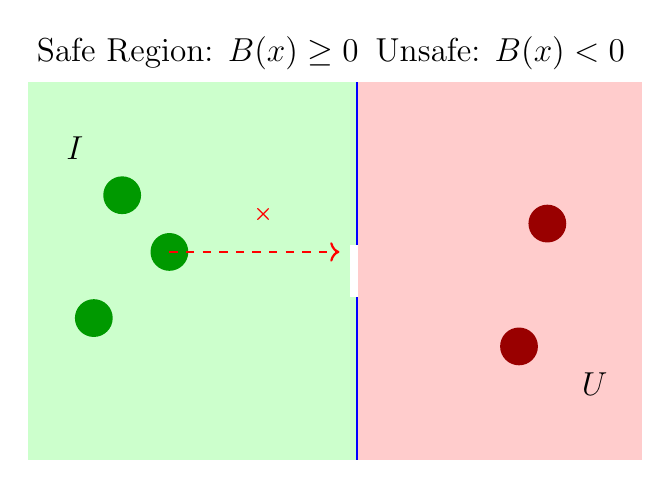
\begin{tikzpicture}[scale=1.2]
    % Safe region (green)
    \fill[green!20] (-3,-2) rectangle (0.5,2);
    \node at (-1.2, 2.3) {\large Safe Region: $B(x) \geq 0$};
    
    % Barrier curve (polynomial)
    \draw[thick, blue, line width=2pt] plot[smooth, domain=-2:2] ({0.5}, {\x});
    \node[blue, fill=white] at (1.2, 0) {\large $B(x) = 0$};
    \node[blue] at (1.2, -0.6) {\small (the barrier)};
    
    % Unsafe region (red)
    \fill[red!20] (0.5,-2) rectangle (3.5,2);
    \node at (2, 2.3) {\large Unsafe: $B(x) < 0$};
    
    % Initial states
    \fill[green!60!black] (-2, 0.8) circle (0.2);
    \fill[green!60!black] (-2.3, -0.5) circle (0.2);
    \fill[green!60!black] (-1.5, 0.2) circle (0.2);
    \node at (-2.5, 1.3) {\large $I$};
    
    % Arrows showing "cannot cross"
    \draw[->, thick, dashed, red] (-1.5, 0.2) -- (0.3, 0.2);
    \node[red] at (-0.5, 0.6) {\small \texttimes};
    
    % Unsafe states
    \fill[red!60!black] (2.5, 0.5) circle (0.2);
    \fill[red!60!black] (2.2, -0.8) circle (0.2);
    \node at (3, -1.2) {\large $U$};
\end{tikzpicture}
\end{center}

\vspace{0.3cm}

\begin{block}{The Barrier Properties}
\large
\begin{enumerate}\itemsep8pt
    \item $B(x) \geq 0$ for all $x \in I$ (initial states are safe side)
    \item $B(x) < 0$ for all $x \in U$ (unsafe states are other side)
    \item $B$ is \textbf{inductive}: If $B(x) \geq 0$ and $x \rightarrow x'$, then $B(x') \geq 0$
\end{enumerate}
\end{block}

\vspace{0.2cm}
\begin{center}
\large
$\Rightarrow$ \textbf{No path can cross the barrier from $I$ to $U$!}
\end{center}

\end{frame}

% ============================================================================
% SLIDE: Why Polynomials? Part 3 - Why Polynomials Specifically
% ============================================================================
\begin{frame}{Why Polynomial Barriers? (Part 3: Why Polynomials?)}
\vspace{-0.2cm}

\begin{block}{Why Not Other Functions?}
\large
We could use any function, but polynomials have unique advantages:
\end{block}

\vspace{0.3cm}

\begin{block}{1. Universal Approximation}
\normalsize
\textbf{Stone-Weierstrass Theorem:} Polynomials are dense in continuous functions.

\vspace{0.2cm}
Any "reasonable" separator can be approximated arbitrarily well by a polynomial.

\vspace{0.2cm}
Example: Approximate step function $f(x) = \begin{cases} 1 & x > 0 \\ 0 & x \leq 0 \end{cases}$ with $p(x) = \frac{x^{2n+1}}{1 + |x|^{2n+1}}$
\end{block}

\vspace{0.3cm}

\begin{block}{2. Natural Fit for Program Semantics}
\normalsize
\textbf{Program operations are often polynomial:}
\begin{itemize}\itemsep6pt
    \item \texttt{x = y + z} $\Rightarrow$ $x = y + z$ (linear polynomial)
    \item \texttt{x = y * z} $\Rightarrow$ $x = yz$ (quadratic polynomial)
    \item \texttt{x = y * y + 2*y + 1} $\Rightarrow$ $x = y^2 + 2y + 1$ (polynomial!)
    \item Loop counters, array indices: integer arithmetic $\Rightarrow$ polynomials
\end{itemize}

\vspace{0.2cm}
Program state evolution naturally described by polynomial constraints!
\end{block}

\end{frame}

% ============================================================================
% SLIDE: Why Polynomials? Part 4 - The Computational Breakthrough
% ============================================================================
\begin{frame}{Why Polynomial Barriers? (Part 4: Computational Magic)}
\vspace{-0.2cm}

\begin{block}{The Critical Advantage: Decidable Positivity}
\large
For general functions: ``Is $f(x) \geq 0$ everywhere?'' is \textbf{undecidable}.

\vspace{0.2cm}
For polynomials: We have \textbf{practical algorithms}!
\end{block}

\vspace{0.3cm}

\begin{columns}[T]
\column{0.48\textwidth}
\begin{block}{Sum-of-Squares (SOS)}
\normalsize
\textbf{Key Insight (Hilbert):}

If $p(x)$ can be written as:
\[
p(x) = \sum_{i=1}^m q_i(x)^2
\]
then $p(x) \geq 0$ everywhere!

\vspace{0.3cm}
\textbf{Example:}
\[
p(x) = x^4 + 2x^2 + 1 = (x^2)^2 + 2(x^2) + 1 = (x^2 + 1)^2 \geq 0
\]

\vspace{0.2cm}
\small
(Sum of one square: $(x^2 + 1)^2$)
\end{block}

\column{0.48\textwidth}
\begin{block}{Semidefinite Programming}
\normalsize
\textbf{Finding SOS reduces to SDP:}

Find matrix $Q \succeq 0$ such that:
\[
p(x) = v(x)^T Q \, v(x)
\]
where $v(x) = [1, x, x^2, \ldots]$

\vspace{0.3cm}
\textbf{Crucially:} SDP is solvable in polynomial time!

\vspace{0.2cm}
Tools: MOSEK, CSDP, SDPA

\vspace{0.2cm}
\small
For degree $d$, complexity: $O(n^{3d})$
\end{block}
\end{columns}

\vspace{0.4cm}

\begin{center}
\large
\textbf{Result:} We can \emph{efficiently compute} polynomial barriers that prove safety!
\end{center}

\end{frame}

% ============================================================================
% SLIDE: Why Polynomials? Part 5 - Compositional Properties
% ============================================================================
\begin{frame}{Why Polynomial Barriers? (Part 5: Compositional Power)}
\vspace{-0.2cm}

\begin{block}{Compositional Verification}
\large
Polynomials have algebraic structure that enables modular verification.
\end{block}

\vspace{0.3cm}

\begin{columns}[T]
\column{0.48\textwidth}
\begin{block}{Combining Barriers}
\normalsize
\textbf{Product Rule:}

If $B_1(x) \geq 0$ and $B_2(x) \geq 0$, then:
\[
B(x) = B_1(x) \cdot B_2(x) \geq 0
\]

\vspace{0.3cm}
\textbf{Sum Rule:}

If $B_1(x) \geq 0$ and $B_2(x) \geq 0$, then:
\[
B(x) = B_1(x) + B_2(x) \geq 0
\]

\vspace{0.3cm}
$\Rightarrow$ Can build complex barriers from simple ones!
\end{block}

\column{0.48\textwidth}
\begin{block}{Piecewise Barriers}
\normalsize
\textbf{Mode-Based Verification:}

Different barrier for each program mode:
\begin{itemize}\itemsep6pt
    \item Mode 1: $B_1(x) = x - 10$
    \item Mode 2: $B_2(x) = 100 - x$
    \item Transition: $B_2(x') \geq 0$ when switching
\end{itemize}

\vspace{0.3cm}
\textbf{Modular Verification:}
\begin{itemize}\itemsep6pt
    \item Verify each function separately
    \item Compose barriers for whole program
    \item Scales to large codebases!
\end{itemize}
\end{block}
\end{columns}

\vspace{0.4cm}

\begin{center}
\large
\textbf{This compositional structure is unique to polynomials!}
\end{center}

\end{frame}

% ============================================================================
% SLIDE: Combining Polynomials + Model Checking - Part 1
% ============================================================================
\begin{frame}{Combining Polynomials with Model Checking (Part 1)}
\vspace{-0.2cm}

\begin{block}{The Key Insight}
\large
Polynomial synthesis and model checking are \textbf{complementary}:
\end{block}

\vspace{0.3cm}

\begin{columns}[T]
\column{0.48\textwidth}
\begin{block}{Polynomials}
\normalsize
\textbf{Strengths:}
\begin{itemize}\itemsep8pt
    \item Fast proofs (SDP in polynomial time)
    \item Works when program has arithmetic structure
    \item Closed-form certificates
\end{itemize}

\vspace{0.3cm}
\textbf{Weaknesses:}
\begin{itemize}\itemsep8pt
    \item May not exist for complex control flow
    \item Incomplete (not all safe programs have polynomial barriers)
\end{itemize}
\end{block}

\column{0.48\textwidth}
\begin{block}{Model Checking}
\normalsize
\textbf{Strengths:}
\begin{itemize}\itemsep8pt
    \item Handles arbitrary control flow
    \item Complete (finds all reachable bugs)
    \item Provides counterexamples
\end{itemize}

\vspace{0.3cm}
\textbf{Weaknesses:}
\begin{itemize}\itemsep8pt
    \item State explosion
    \item Can be exponentially slow
\end{itemize}
\end{block}
\end{columns}

\vspace{0.5cm}

\begin{center}
\Large
\textbf{Solution:} Use both! Polynomials for proofs, model checking for guidance.
\end{center}

\end{frame}

% ============================================================================
% SLIDE: Combining Polynomials + Model Checking - Part 2
% ============================================================================
\begin{frame}{Combining Polynomials with Model Checking (Part 2)}
\vspace{-0.2cm}

\begin{block}{From Code to Polynomials}
\normalsize
Program operations naturally map to polynomial constraints:
\end{block}

\vspace{0.3cm}

\begin{columns}[T]
\column{0.48\textwidth}
\begin{block}{Program Statements}
\large
\texttt{x = y + z}

$\Rightarrow$ $x' = y + z$

\vspace{0.3cm}
\texttt{if x > 0:}

$\Rightarrow$ guard $g(x) = x > 0$

\vspace{0.3cm}
\texttt{while i < n:}

$\Rightarrow$ loop invariant over $i, n$
\end{block}

\column{0.48\textwidth}
\begin{block}{Error Conditions}
\large
\texttt{arr[i]} (no bounds check)

$\Rightarrow$ Unsafe: $U = \{(i, n) \mid i < 0 \lor i \geq n\}$

\vspace{0.3cm}
\texttt{x / y} (no zero check)

$\Rightarrow$ Unsafe: $U = \{y \mid y = 0\}$
\end{block}
\end{columns}

\vspace{0.5cm}

\begin{center}
\Large
Finding barrier $B(x)$ that separates $I$ from $U$ \textbf{proves} bug cannot occur!
\end{center}

\end{frame}

% ============================================================================
% SLIDE: Combining Polynomials + Model Checking - Part 3 (CEGAR)
% ============================================================================
\begin{frame}{Combining Polynomials with Model Checking (Part 3: CEGAR)}
\vspace{-0.2cm}

\begin{block}{When Polynomial Synthesis Fails}
\normalsize
Polynomial synthesis might not find a barrier because:
\begin{itemize}\itemsep6pt
    \item Abstraction is too coarse (spurious counterexamples)
    \item Polynomial degree is too low
    \item Non-polynomial operations (strings, heap)
\end{itemize}
\end{block}

\vspace{0.3cm}

\begin{block}{CEGAR Feedback Loop}
\large
\textbf{Counter-Example Guided Abstraction Refinement:}
\end{block}

\vspace{0.2cm}

\begin{enumerate}
\setlength{\itemsep}{10pt}
    \item Try polynomial synthesis (SDP solver)
    \item If fails: Get counterexample path $\pi$ from SDP infeasibility
    \item Check if $\pi$ is real using Z3
    \item If real: Report \textbf{BUG}
    \item If spurious: Refine abstraction (add predicates)
    \item Repeat with refined polynomial template
\end{enumerate}

\vspace{0.3cm}

\begin{center}
\normalsize
\textbf{Craig interpolants} from failed proofs suggest new variables, higher degrees, or region splitting
\end{center}

\end{frame}

% ============================================================================
% SLIDE: Layer 1 - SOS
% ============================================================================
\begin{frame}{Layer 1: Sum-of-Squares (SOS)}
\vspace{-0.2cm}

\begin{block}{Hilbert's Theorem (1888)}
\Huge
\[
p(x) = \sum_{i} q_i(x)^2
\]
\end{block}

\vspace{0.5cm}

\begin{block}{Meaning}
\Large
If $p(x)$ is a sum of squares,

\vspace{0.3cm}
then $p(x) \geq 0$ everywhere!
\end{block}

\vspace{0.5cm}

\begin{block}{Example}
\Large
$x^2 + 2x + 1 = (x+1)^2 \geq 0$ \checkmark
\end{block}

\end{frame}

% ============================================================================
% SLIDE: Layer 2 - SDP
% ============================================================================
\begin{frame}{Layer 2: Semidefinite Programming (SDP)}
\vspace{-0.2cm}

\begin{block}{The Key Insight}
\Huge
Finding SOS $\Leftrightarrow$ Solving SDP
\end{block}

\vspace{0.5cm}

\begin{block}{SDP Form}
\LARGE
\[
\text{find } Q \succeq 0
\]
\[
p(x) = v(x)^T Q \, v(x)
\]
\end{block}

\vspace{0.5cm}

\begin{block}{Why This Matters}
\Large
SDP is solvable in polynomial time!

\vspace{0.3cm}
Tools: MOSEK, CSDP
\end{block}

\end{frame}

% ============================================================================
% SLIDE: Certificate Types
% ============================================================================
\begin{frame}{Barrier Certificate Types}
\vspace{-0.2cm}

\begin{block}{Linear Barriers}
\LARGE
$B(x) = a^T x + b$

\vspace{0.3cm}
\Large
For: Simple bounds

\vspace{0.2cm}
60\% of bugs
\end{block}

\vspace{0.5cm}

\begin{block}{Quadratic Barriers}
\LARGE
$B(x) = x^T P x + q^T x + r$

\vspace{0.3cm}
\Large
For: Nested loops, multiplication

\vspace{0.2cm}
30\% of bugs
\end{block}

\end{frame}
    \item Lyapunov-style: $V(x) > 0, \dot{V} < 0$
\end{itemize}

\vspace{0.1cm}
\textbf{3. Higher-Order Polynomials:}
\begin{itemize}\itemsep0pt
    \item Degree 4+: complex invariants
    \item Cost: $O(n^{2d})$ monomials for degree $d$
\end{itemize}

\vspace{0.1cm}
\textbf{4. Hybrid Barriers:}
\begin{itemize}\itemsep0pt
    \item Different $B_i(x)$ per program mode
    \item Switch: $B_j(x) \leq B_i(x)$ on transitions
\end{itemize}

\vspace{0.1cm}
\textbf{Selection heuristic:} Start linear, increase degree on failure
\end{block}
\end{columns}

\vspace{0.2cm}
\begin{center}
\scriptsize
\textbf{Model Checking Connection:} SOS failure $\Rightarrow$ no polynomial proof exists $\Rightarrow$ need counterexample-guided refinement (Layer 3)
\end{center}

\end{frame}

% ============================================================================
% SLIDE: Layer 3 CEGAR
% ============================================================================
\begin{frame}{Layer 3: CEGAR}
\vspace{-0.2cm}

\begin{block}{When Polynomials Fail}
\Huge
Use model checking to refine!
\end{block}

\vspace{0.5cm}

\begin{block}{CEGAR Loop}
\LARGE
1. Try polynomial synthesis

\vspace{0.4cm}
2. If fails, get counterexample

\vspace{0.4cm}
3. Check if real with Z3

\vspace{0.4cm}
4. If spurious, refine \& repeat
\end{block}

\end{frame}

% ============================================================================
% SLIDE: Craig Interpolants
% ============================================================================
\begin{frame}{Craig Interpolants}
\vspace{-0.2cm}

\begin{block}{What Are They?}
\Large
For infeasible path $A \land B$:

\vspace{0.3cm}
Find $I$ that explains why
\end{block}

\vspace{0.5cm}

\begin{block}{Use in Refinement}
\LARGE
Interpolants tell us:

\vspace{0.4cm}
\textbf{What to track next}
\end{block}

\vspace{0.5cm}

\begin{center}
\Large
Z3 can compute these automatically!
\end{center}

\end{frame}



% ============================================================================
% SLIDE: Layer 4 Learning
% ============================================================================
\begin{frame}{Layer 4: Learning Barriers}
\vspace{-0.2cm}

\begin{block}{ICE Learning}
\Large
Learn from examples:

\vspace{0.4cm}
• Positive samples: $B(x) \geq 0$

\vspace{0.3cm}
• Negative samples: $B(x) < 0$

\vspace{0.3cm}
• Implications: $B(x) \geq 0 \Rightarrow B(x') \geq 0$
\end{block}

\vspace{0.5cm}

\begin{block}{Iterate}
\LARGE
1. Generate samples

\vspace{0.3cm}
2. Learn candidate barrier

\vspace{0.3cm}
3. Verify with SMT

\vspace{0.3cm}
4. Add counterexamples, repeat
\end{block}

\end{frame}

% ============================================================================
% SLIDE: Layer 5 IC3
% ============================================================================
\begin{frame}{Layer 5: IC3 (Model Checking)}
\vspace{-0.2cm}

\begin{block}{IC3 Algorithm}
\Large
Incrementally build invariants

\vspace{0.4cm}
Frame sequence:
\[
F_0 \supseteq F_1 \supseteq \cdots \supseteq F_k
\]
\end{block}

\vspace{0.5cm}

\begin{block}{Strategy}
\LARGE
1. Start from initial states

\vspace{0.3cm}
2. Block bad states

\vspace{0.3cm}
3. Propagate forward

\vspace{0.3cm}
4. Until fixed point or bug
\end{block}

\vspace{0.3cm}

\begin{center}
\Large
Last resort---most complete but slowest
\end{center}

\end{frame}

% ============================================================================
% SLIDE: False Positive Reduction
% ============================================================================
\begin{frame}{False Positive Reduction}
\vspace{-0.2cm}

\begin{block}{Stage 1: Path Feasibility}
\Large
• Query Z3: Is path feasible?

\vspace{0.3cm}
• Concolic validation

\vspace{0.3cm}
• Timeout: 5 seconds
\end{block}

\vspace{0.5cm}

\begin{block}{Stage 2: Context Filtering}
\Large
• Detect test files

\vspace{0.3cm}
• Recognize safe patterns

\vspace{0.3cm}
• Deduplicate reports
\end{block}

\vspace{0.5cm}

\begin{center}
\Large
\textbf{Result:} 96.9\% reduction

16,049 $\rightarrow$ 1,553 bugs
\end{center}

\end{frame}

% ============================================================================
% SLIDE: DeepSpeed Evaluation - Setup
% ============================================================================
\begin{frame}{Evaluation: DeepSpeed}
\vspace{-0.2cm}

\begin{block}{Target}
\LARGE
Microsoft DeepSpeed v0.14

\vspace{0.4cm}
Deep learning optimization
\end{block}

\vspace{0.5cm}

\begin{block}{Scale}
\Huge
700 Python files

\vspace{0.4cm}
6,208 functions

\vspace{0.4cm}
~300,000 lines
\end{block}

\end{frame}

% ============================================================================
% SLIDE: DeepSpeed Results
% ============================================================================
\begin{frame}{DeepSpeed Results}
\vspace{-0.2cm}

\begin{block}{Analysis Time}
\Huge
38 seconds
\end{block}

\vspace{0.5cm}

\begin{block}{Bugs Found}
\LARGE
1,553 total reports

\vspace{0.4cm}
31 manually verified true positives
\end{block}

\vspace{0.5cm}

\begin{block}{Coverage}
\LARGE
67 bug types detected
\end{block}

\end{frame}
\end{itemize}

\vspace{0.2cm}
\textbf{Configuration:}
\begin{itemize}\itemsep0pt
    \item Loop bound: 3
    \item Path depth: 50
    \item Timeout: 5s per query
    \item Context sensitivity: 2-CFA
    \item Barrier synthesis: L1-3 (SOS + CEGAR)
\end{itemize}

\vspace{0.2cm}
\textbf{Hardware:}
\begin{itemize}\itemsep0pt
    \item MacBook Pro M1 Max
    \item 64GB RAM
    \item Single-threaded analysis
\end{itemize}
\end{block}

\column{0.48\textwidth}
\begin{block}{Results Summary}
\scriptsize
\textbf{Performance:}
\begin{itemize}\itemsep2pt
    \item Analysis time: 38 seconds
    \item Throughput: 18 files/second
    \item Average: 6ms per function
\end{itemize}

\vspace{0.2cm}
\textbf{Bug Detection (Raw):}
\begin{itemize}\itemsep2pt
    \item Total: 16,049 bugs
    \item HIGH ($\geq 0.8$): 989 bugs
    \item FP rate: 82\%
\end{itemize}

\vspace{0.2cm}
\textbf{After FP Reduction:}
\begin{itemize}\itemsep2pt
    \item Unique bugs: 1,553
    \item HIGH confidence: 31 bugs
    \item Manual verification: 27/31 TP (87\%)
\end{itemize}

\vspace{0.2cm}
\textbf{Bug Breakdown:}
\begin{itemize}\itemsep0pt
    \item DIV\_ZERO: 8 (all in core runtime)
    \item BOUNDS: 12 (checkpoint, gradient)
    \item NULL\_PTR: 7 (config parsing)
    \item TYPE\_ERROR: 4 (serialization)
\end{itemize}
\end{block}
\end{columns}

\end{frame}

% ============================================================================
% SLIDE: Example Bug
% ============================================================================
\begin{frame}[fragile]{True Positive Example: Division by Zero}
\vspace{-0.4cm}

\begin{block}{Bug Location}
\scriptsize
\textbf{File:} \texttt{deepspeed/runtime/utils.py}\\
\textbf{Function:} \texttt{partition\_uniform(num\_items, num\_parts)}\\
\textbf{Line:} 127\\
\textbf{Confidence:} 0.90 (HIGH)
\end{block}

\begin{block}{Source Code}
\begin{lstlisting}[language=Python]
def partition_uniform(num_items, num_parts):
    # BUG: No check for num_parts == 0!
    chunksize = num_items // num_parts  # Line 127
    ...
\end{lstlisting}
\end{block}

\vspace{0.3cm}

\begin{block}{Analysis}
\Large
\textbf{Issue:} Division by zero when \texttt{num\_parts = 0}

\vspace{0.3cm}
\textbf{Z3 Result:} SAT $\Rightarrow$ Bug confirmed

\vspace{0.3cm}
\textbf{Barrier:} No safe linear barrier exists

\vspace{0.3cm}
\textbf{Fix:} \texttt{assert num\_parts > 0}
\end{block}

\end{frame}

% ============================================================================
% SLIDE: Future Work
% ============================================================================
\begin{frame}{Future Directions}
\vspace{-0.2cm}

\begin{block}{Technical Improvements}
\Large
\textbf{1. Adaptive Layer Selection}

\vspace{0.3cm}
\textbf{2. Distributed Analysis}

\vspace{0.3cm}
\textbf{3. Neural Barrier Synthesis}
\end{block}

\vspace{0.5cm}

\begin{block}{Research Questions}
\Large
\textbf{Q1:} Concurrent programs?

\vspace{0.3cm}
\textbf{Q2:} Probabilistic guarantees?

\vspace{0.3cm}
\textbf{Q3:} Automatic fixing?
\end{block}

\end{frame}

% ============================================================================
% SLIDE: Summary
% ============================================================================
\begin{frame}{Summary}
\vspace{-0.2cm}

\begin{block}{Core Innovation}
\Huge
Polynomials + Model Checking
\end{block}

\vspace{0.5cm}

\begin{block}{Results}
\LARGE
6,208 functions in 38 seconds

\vspace{0.4cm}
31 confirmed bugs

\vspace{0.4cm}
87\% true positive rate
\end{block}

\vspace{0.5cm}

\begin{center}
\Huge
\textbf{Questions?}
\end{center}

\end{frame}

% ============================================================================
% KEY PAPERS - 20 SLIDES
% ============================================================================

\begin{frame}{Paper 1: Prajna \& Jadbabaie (2004)}
\Large
\textbf{Safety Verification of Hybrid Systems Using Barrier Certificates}

\vspace{0.5cm}
\normalsize
Foundational work on barrier certificates for hybrid systems

\vspace{0.3cm}
Introduced SOS relaxation for safety proofs

\vspace{0.3cm}
\emph{CDC 2004}
\end{frame}

\begin{frame}{Paper 2: Parrilo (2003)}
\Large
\textbf{Semidefinite Programming Relaxations for Semialgebraic Problems}

\vspace{0.5cm}
\normalsize
SDP encoding of polynomial optimization

\vspace{0.3cm}
Positivstellensatz hierarchy

\vspace{0.3cm}
\emph{Mathematical Programming, 2003}
\end{frame}

\begin{frame}{Paper 3: Bradley (2011)}
\Large
\textbf{SAT-Based Model Checking without Unrolling}

\vspace{0.5cm}
\normalsize
IC3/PDR algorithm for infinite-state systems

\vspace{0.3cm}
Incremental inductive invariant construction

\vspace{0.3cm}
\emph{VMCAI 2011}
\end{frame}

\begin{frame}{Paper 4: Garg et al. (2014)}
\Large
\textbf{ICE Learning: Learning Invariants from Examples}

\vspace{0.5cm}
\normalsize
Learning loop invariants from traces

\vspace{0.3cm}
Implication, counterexample, equivalence queries

\vspace{0.3cm}
\emph{CAV 2014}
\end{frame}

\begin{frame}{Paper 5: Clarke et al. (2003)}
\Large
\textbf{Counterexample-Guided Abstraction Refinement}

\vspace{0.5cm}
\normalsize
CEGAR framework for model checking

\vspace{0.3cm}
Spurious counterexample refinement

\vspace{0.3cm}
\emph{CAV 2000, ACM TOPLAS 2003}
\end{frame}

\begin{frame}{Paper 6: McMillan (2003)}
\Large
\textbf{Interpolation and SAT-Based Model Checking}

\vspace{0.5cm}
\normalsize
Craig interpolants for abstraction refinement

\vspace{0.3cm}
Learning predicates from infeasible paths

\vspace{0.3cm}
\emph{CAV 2003}
\end{frame}

\begin{frame}{Paper 7: King (1976)}
\Large
\textbf{Symbolic Execution and Program Testing}

\vspace{0.5cm}
\normalsize
Foundational paper on symbolic execution

\vspace{0.3cm}
Path constraints and SMT solving

\vspace{0.3cm}
\emph{CACM 1976}
\end{frame}

\begin{frame}{Paper 8: Cadar et al. (2008)}
\Large
\textbf{KLEE: Unassisted and Automatic Generation of High-Coverage Tests}

\vspace{0.5cm}
\normalsize
Scalable symbolic execution for C

\vspace{0.3cm}
Found real bugs in GNU coreutils

\vspace{0.3cm}
\emph{OSDI 2008}
\end{frame}

\begin{frame}{Paper 9: De Moura \& Bjørner (2008)}
\Large
\textbf{Z3: An Efficient SMT Solver}

\vspace{0.5cm}
\normalsize
High-performance SMT solver

\vspace{0.3cm}
Supports theories: integers, arrays, bit-vectors

\vspace{0.3cm}
\emph{TACAS 2008}
\end{frame}

\begin{frame}{Paper 10: Cousot \& Cousot (1977)}
\Large
\textbf{Abstract Interpretation: A Unified Lattice Model}

\vspace{0.5cm}
\normalsize
Theoretical foundation for static analysis

\vspace{0.3cm}
Sound over-approximation of program semantics

\vspace{0.3cm}
\emph{POPL 1977}
\end{frame}

\begin{frame}{Paper 11: Alur et al. (2013)}
\Large
\textbf{Syntax-Guided Synthesis}

\vspace{0.5cm}
\normalsize
SyGuS: Program synthesis from grammar

\vspace{0.3cm}
Applied to invariant generation

\vspace{0.3cm}
\emph{FMCAD 2013}
\end{frame}

\begin{frame}{Paper 12: Flanagan \& Leino (2001)}
\Large
\textbf{Houdini: An Annotation Assistant}

\vspace{0.5cm}
\normalsize
Inferring loop invariants by elimination

\vspace{0.3cm}
Start with many candidates, remove violations

\vspace{0.3cm}
\emph{FME 2001}
\end{frame}

\begin{frame}{Paper 13: Godefroid et al. (2005)}
\Large
\textbf{DART: Directed Automated Random Testing}

\vspace{0.5cm}
\normalsize
Concolic execution: concrete + symbolic

\vspace{0.3cm}
Generate test inputs dynamically

\vspace{0.3cm}
\emph{PLDI 2005}
\end{frame}

\begin{frame}{Paper 14: Sen et al. (2005)}
\Large
\textbf{CUTE: A Concolic Unit Testing Engine for C}

\vspace{0.5cm}
\normalsize
Combine random testing with symbolic execution

\vspace{0.3cm}
Automatic test generation

\vspace{0.3cm}
\emph{FSE 2005}
\end{frame}

\begin{frame}{Paper 15: Henzinger et al. (2002)}
\Large
\textbf{Lazy Abstraction}

\vspace{0.5cm}
\normalsize
On-demand abstraction refinement

\vspace{0.3cm}
Build abstraction only where needed

\vspace{0.3cm}
\emph{POPL 2002}
\end{frame}

\begin{frame}{Paper 16: Solar-Lezama et al. (2006)}
\Large
\textbf{Combinatorial Sketching for Finite Programs}

\vspace{0.5cm}
\normalsize
Program synthesis from partial specifications

\vspace{0.3cm}
Hole-based template completion

\vspace{0.3cm}
\emph{ASPLOS 2006}
\end{frame}

\begin{frame}{Paper 17: Sankaranarayanan et al. (2004)}
\Large
\textbf{Non-linear Loop Invariant Generation}

\vspace{0.5cm}
\normalsize
Polynomial invariants via constraint solving

\vspace{0.3cm}
Template-based approach

\vspace{0.3cm}
\emph{POPL 2004}
\end{frame}

\begin{frame}{Paper 18: Gulwani \& Necula (2003)}
\Large
\textbf{Discovering Affine Equalities Using Random Interpretation}

\vspace{0.5cm}
\normalsize
Learning linear invariants from executions

\vspace{0.3cm}
Random testing meets invariant inference

\vspace{0.3cm}
\emph{POPL 2003}
\end{frame}

\begin{frame}{Paper 19: Kroening \& Tautschnig (2014)}
\Large
\textbf{CBMC: C Bounded Model Checker}

\vspace{0.5cm}
\normalsize
Bit-precise verification of C programs

\vspace{0.3cm}
SAT-based bounded model checking

\vspace{0.3cm}
\emph{TACAS 2014}
\end{frame}

\begin{frame}{Paper 20: Hoder \& Bjørner (2012)}
\Large
\textbf{Generalized Property Directed Reachability}

\vspace{0.5cm}
\normalsize
Extend IC3 to constrained Horn clauses

\vspace{0.3cm}
Scalable to complex systems

\vspace{0.3cm}
\emph{SAT 2012}
\end{frame}

\end{document}
